\section{Kupfer-PVD}
\label{copperpvd}

Anhand von Kupfer-PVD wurde die Abscheidung eines weiteren fcc-Metalls mit Parsivald simuliert, wofür zuvor verschiedene EAM-Parametersätze untersucht wurden (Tabelle~\ref{tab:copperpots}).
Für diese Parametersätze wird eine kurze Voruntersuchung durchgeführt, bevor mit einer kleinen Auswahl von ihnen Abscheidungsprozesse mit Parsivald simuliert werden.

\begin{table}[bhp]
  \oddrowcolors
  \caption{Untersuchte EAM-Parametrisierungen für Kupfersysteme}
  \label{tab:copperpots}
  \begin{tabularx}{\textwidth}{|lXc|}
    \hline
    \textbf{Bezeichnung}                  & \textbf{Anwendung \& Kommentare}                                            & \textbf{Ref.}                           \\
    \hline
    \pot{CuAg.eam.alloy}                  & struktur. und thermodyn. Eigenschaften von \ce{Cu-Ag}                       & \cite{williams_embedded-atom_2006}      \\
    \pot{cu\_ag\_ymwu.eam.alloy}          & Mono-, Di-, Trimere und Inseln von \ce{Cu} auf \ce{Ag}                      & \cite{wu_cu/ag_2009}                    \\
    \pot{Cu\_smf7.eam} \qquad(\pot{smf7}) & Oberflächen von \ce{Ni-Cu}-Legierungen bei \SI{800}{\kelvin}                & \cite{foiles_calculation_1985}          \\
    \pot{Cu\_u3.eam} \qqquad(\pot{u3})    & fcc-Metalle und Legierungen                                                 & \cite{foiles_embedded-atom-method_1986} \\
    \pot{Cu\_u6.eam} \qqquad(\pot{u6})    & Aktivierungsenergie für Eigendiffusionen                                    & \cite{adams_self-diffusion_1989}        \\
    \pot{Cu-Zr\_2.eam.fs}                 & Flüssige und amorphe \ce{Cu-Zr}-Legierungen                                 & \cite{mendelev_development_2009}        \\
    \pot{Cu-Zr.eam.fs}                    & Flüssige und amorphe \ce{Cu-Zr}-Legierungen                                 & \cite{mendelev_using_2007}              \\
    \pot{Mendelev\_Cu2.eam.fs}            & Unterkühlte \ce{Al-Cu}-Schmelzen. Basiert auf \cite{mendelev_analysis_2008} & \cite{becker_interatomic_2014}          \\
    \hline
  \end{tabularx}

\end{table}

\subsection{Voruntersuchungen}

Die untersuchten Parametersätze unterscheiden sich in ihren beabsichtigten Anwendungszwecken, die von der Darstellung von kristallinem Kupfer über Legierungen bis zu Metallschmelzen reichen.
Wie bei den Voruntersuchungen für Gold-PVD zuvor (Abschnitt~\ref{goldpreparation}) wurde eine Bestimmung der Koordinationszahl, Bindungslänge und Dichte von kristallinem Kupfer durchgeführt und die erhaltenen Werte mit Literaturwerten\cite{haynes_crc_2011} verglichen.

\begin{table}[b!]
  \begin{threeparttable}
    \oddrowcolors
    \caption{Vergleich struktureller Eigenschaften von Kupfer mit Literaturdaten}
    \label{tab:copperpreresults}
    \begin{tabularx}{\textwidth}{|Xrrrrr|}
      \hline
      \textbf{Parametersatz}       & \textbf{Koord.} & \multicolumn{2}{c}{\textbf{Bindungslänge}}     & \textbf{Dichte}   & ~                      \\
      \hline
      Referenz                     & \num{12.00}     & \SI{2.556}{\angstrom} & ~                      & \SI{8.96}{\gpcc}  & ~                      \\
      \pot{CuAg.eam.alloy}         & \num{12.09}     & \SI{2.559}{\angstrom} & (\SI{-0.12}{\percent}) & \SI{8.893}{\gpcc} & (\SI{-0.75}{\percent}) \\
      \pot{cu\_ag\_ymwu.eam.alloy} & \num{12.03}     & \SI{2.473}{\angstrom} & (\SI{-3.25}{\percent}) & \SI{9.846}{\gpcc} & (\SI{+9.89}{\percent}) \\
      \pot{Cu\_smf7.eam}           & \num{12.03}     & \SI{2.558}{\angstrom} & (\SI{+0.08}{\percent}) & \SI{8.908}{\gpcc} & (\SI{-0.58}{\percent}) \\
      \pot{Cu\_u3.eam}             & \num{12.00}     & \SI{2.558}{\angstrom} & (\SI{+0.08}{\percent}) & \SI{8.915}{\gpcc} & (\SI{-0.50}{\percent}) \\
      \pot{Cu\_u6.eam}             & \num{12.00}     & \SI{2.558}{\angstrom} & (\SI{+0.08}{\percent}) & \SI{8.910}{\gpcc} & (\SI{-0.56}{\percent}) \\
      \pot{CuNi.eam.alloy}         & \num{12.10}     & \SI{2.559}{\angstrom} & (\SI{-0.12}{\percent}) & \SI{8.895}{\gpcc} & (\SI{-0.73}{\percent}) \\
      \pot{Cu-Zr\_2.eam.fs}        & \num{12.05}     & \SI{2.575}{\angstrom} & (\SI{-0.74}{\percent}) & \SI{8.738}{\gpcc} & (\SI{-2.48}{\percent}) \\
      \pot{Cu-Zr.eam.fs}           & \num{12.09}     & \SI{2.575}{\angstrom} & (\SI{-0.74}{\percent}) & \SI{8.738}{\gpcc} & (\SI{-2.48}{\percent}) \\
      \pot{Mendelev\_Cu2.eam.fs}   & \num{12.07}     & \SI{2.575}{\angstrom} & (\SI{-0.74}{\percent}) & \SI{8.747}{\gpcc} & (\SI{-2.38}{\percent}) \\
      \hline
    \end{tabularx}

    %% \tnote{a}
    %% \begin{tablenotes}
    %%   \item[a] Der Wert in Klammern ist die Abweichung vom experimentellen Wert
    %% \end{tablenotes}
  \end{threeparttable}
\end{table}

Die Ergebnisse stimmen gut mit Literaturwerten überein (Tabelle~\ref{tab:copperpreresults}), zeigen aber eine größere Abweichung für \pot{cu\_ag\_ymwu.eam.alloy}, die sich wahrscheinlich aus der beabsichtigten Anwendung für nanoskopische Kupfer-Partikel anstelle von Bulkmaterialien resultiert.
Die anderen Parametersätze zeigen für die Dichte und die Bindungslänge eine Abweichung unterhalb von \SI{1}{\percent}, wobei die mit LAMMPS verbreiteten Dateien \pot{smf7}, \pot{u3} und \pot{u6} ideale strukturelle Eigenschaften beschreiben.
Da diese drei Parametersätze, welche von der Arbeitsgruppe um \textsc{S.~M.~Foiles}\cite{foiles_calculation_1985,foiles_embedded-atom-method_1986,adams_self-diffusion_1989} stammen, auf die Beschreibung von fcc-Metallen, ihren Oberflächen und Legierungen ausgelegt sind, werden sie in den nachfolgenden Parsivald-Simulationen genutzt.

\subsection{Thermodynamische Eigenschaften}

Wie für Gold zuvor (Abschnitt~\ref{goldthermo}) wurde auch für die Kupfer-Parametersätze eine Untersuchung der thermodynamischen Eigenschaften durchgeführt.
Dabei zeigt sich für die meisten Parametersätze mit Ausnahme von \pot{cu\_ag\_ymwu.eam.alloy} eine Überschätzung der Schmelztemperatur um ca. \SI{200}{\kelvin} (Abbildung~\ref{fig:copperthermo}).

Daran ist die Eigenschaft von MD-Potentialen erkennbar, nach der Parametrisierungen für die Beschreibung struktureller Eigenschaften in der Regel keine thermodynamischen Eigenschaften darstellen.
Unterhalb von \SI{1000}{\kelvin} stimmen die meisten Dichten mit Referenzwerten überein, die über den linearen Ausdehnungskoeffizienten von $\alpha = \SI{16.5e-6}{\per\kelvin}$\cite{haynes_crc_2011} berechnet wurden, weshalb die geringen Abscheidungstemperaturen von \SI{500}{\kelvin} die Schichteigenschaften nicht verfälschen sollten.
Die Referenzwerte stammen aus den Referenzen~\cite{haynes_crc_2011,brillo_density_2006} (Siehe Anhang~\ref{appendix_constants}).

\begin{figure}[H]
  \centering
  \captionsetup[subfigure]{singlelinecheck=false}
  \begin{subfigure}[c]{9.4cm}
    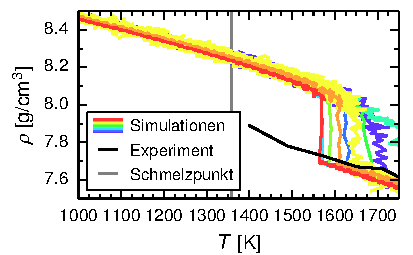
\includegraphics[width=\textwidth]{Cu_u6_meltingpoint}
  \end{subfigure}
  \begin{subfigure}[c]{3cm}
    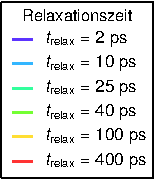
\includegraphics[width=\textwidth]{Cu_u6_meltingpoint_legend}
    \vspace{1.5em}
  \end{subfigure}
  \hfill
  \caption[Vergleich der Schmelztemperatur von Kupfer]{
    Vergleich der Schmelztemperatur von Kupfer.
    Experimentelle Dichte:~\cite{brillo_density_2006}
  }
  \label{fig:copperthermo}
  \todoline{Schriftgröße zwischen beiden Diagrammen anpassen}
\end{figure}

\begin{figure}[H]
  \centering
  \captionsetup[subfigure]{singlelinecheck=false}
  \begin{subfigure}[c]{9.4cm}
    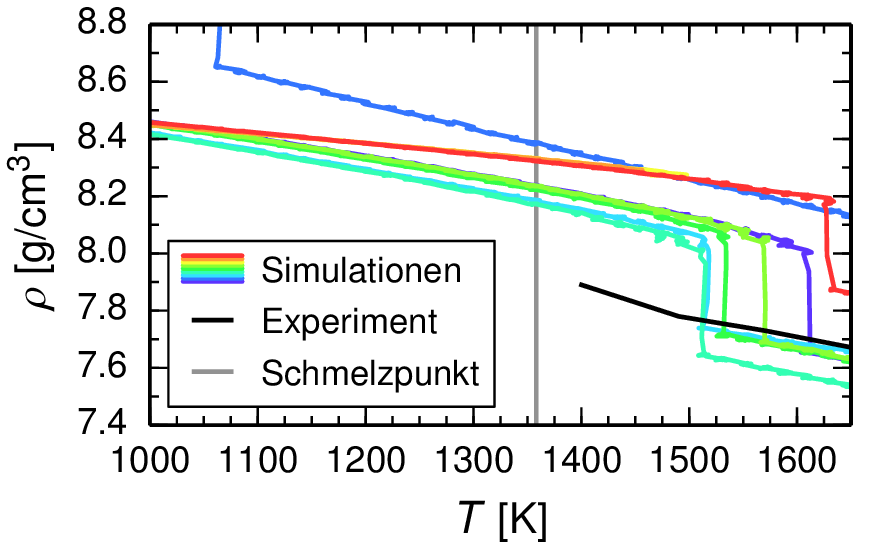
\includegraphics[width=\textwidth]{Cu_trelax_all}
  \end{subfigure}
  \begin{subfigure}[c]{4.7cm}
    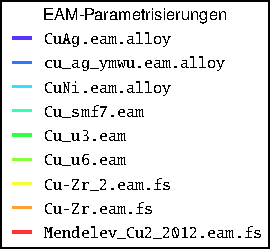
\includegraphics[width=\textwidth]{Cu_trelax_all_legend}
    \vspace{1.5em}
  \end{subfigure}
  \hfill
  \caption[Vergleich der Schmelztemperatur von Kupfer]{
    Vergleich der Schmelztemperatur von Kupfer.
    Experimentelle Dichte:~\cite{brillo_density_2006}
  }
  \label{fig:copperthermo2}
\end{figure}

\subsection{Prozess-Simulation}
\label{coppersimulation}

In einer PVD-Simulation soll zunächst überprüft werden, ob Kupfer im PVD-Modus von Parsivald mit den gleichen Eigenschaften wie für den Gold-Prozess abgeschieden werden kann.
Weiterhin werden die abgeschiedenen Schichten auf Unebenheiten, Fehlstellen und Hohlräume untersucht, um Aussagen über deren Qualität zu gewinnen.
Durch die Ähnlichkeiten zwischen Kupfer und Gold wurden die Prozess-Parameter der Gold-PVD für den Kupfer-Prozess adaptiert.
Unterschiede liegen in den Auftreffenergien von \SI{5.4}{\electronvolt}, die ebenfalls vom Thermostat vor dem eigentlichen Auftreffen der Atome auf der Oberfläche noch weiter abgeschwächt werden.

\begin{figure}[b!]
  \captionsetup[subfigure]{singlelinecheck=false}
  \def\subfigwidth{0.49\textwidth}
  \begin{subfigure}[t]{\subfigwidth}
    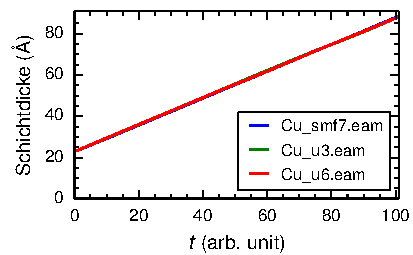
\includegraphics[width=\textwidth]{Cu_thickness}
    \subcaption{Zeitliche Entwicklung der Schichtdicke}
    \label{fig:copperparsivald-a}
  \end{subfigure}
  \hfill
  \begin{subfigure}[t]{\subfigwidth}
    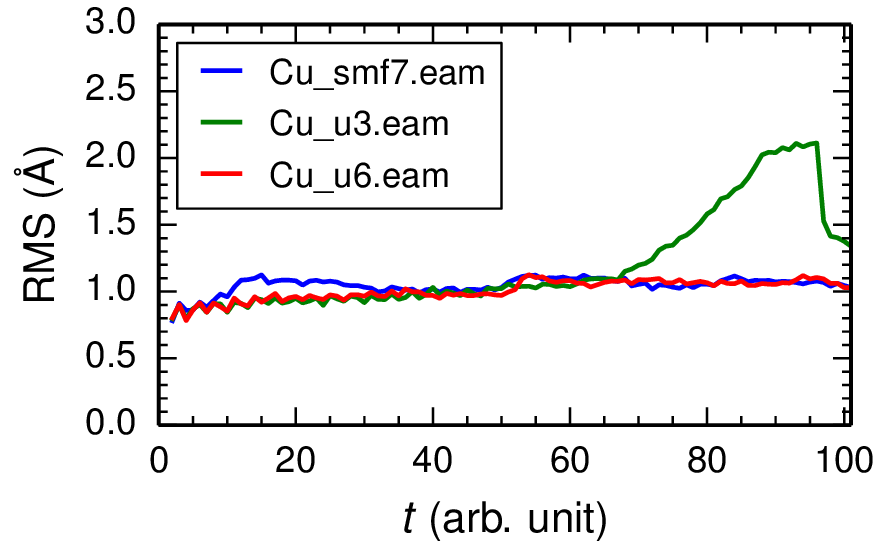
\includegraphics[width=\textwidth]{Cu_roughness}
    \subcaption{Zeitliche Entwicklung der Rauheit}
    \label{fig:copperparsivald-b}
  \end{subfigure}
  \caption{Simulationen von Kupfer-PVD auf \SI{200x200x24}{\angstrom} großen Substraten}
  \label{fig:copperparsivald}
\end{figure}

Auch bei Kupfer-PVD zeigt die Simulation epitaktisches Wachstum glatter Schichten (Abbildungen~\ref{fig:copperparsivald-a} und~\ref{fig:copperparsivald-b}), die bei genauer Prüfung zwar keine Gitter-Fehlstellen, aber gelegentlich einzelne Hohlräume mit einem Durchmesser von ca. \SI{1}{\nano\meter} beinhalten.
Sie bilden sich im Verlauf der Simulation als kraterförmige Vertiefungen auf der Oberfläche, die sich verjüngen, bevor sie von der aufwachsenden Schicht zu Hohlräumen abgeschlossen werden (Abbildung~\ref{fig:coppercrater}).

Betrachtungen der MD-Simulationen für die mit der Kraterbildung verbundenen Ereignisse zeigen, dass bei Ankunft des Gasatomes seine kinetische Energie fast vollständig an ein anderes Teilchen übertragen wird, das dadurch aus der Oberfläche geschlagen wird.
An den betroffenen Abscheidungsorten liegen glatte, perfekt kristalline Oberflächen vor, die sich auch im späteren Simulationsverlauf mit einer geringen Wahrscheinlichkeit bilden können.
Untersuchungen des Einflusses der Teilchenenergie auf den Sputter-Prozess\cite{zhou_atomistic_1998} haben für glatte Oberflächen eine geringere Wahrscheinlichkeit des Energieaustauches gezeigt als für unebene Oberflächen, doch wurden bei diesen Simulationen Energieminimierungen durchgeführt.
Die Kraterbildung sollte so eigentlich von einer atomaren Stufe ausgehen, doch wird die Energie in Parsivald-Simulationen bei unebenen Oberflächen scheinbar besser auf die Oberflächenatome aufgeteilt.

Parsivald kann mit herausgeschlagenen Atomen in der aktuellen Version nicht umgehen, weshalb das Ereignis als fehlgeschlagen markiert wird und in den Abbruchraten (Abbildung~\ref{fig:copperworkerdensity-a}) erkennbar sind, die das Verhältnis von fehlgeschlagenen zu ausgewählten Ereignissen beschreiben.
Die Kraterbildung ist auch in den Rauheiten (Abbildung~\ref{fig:copperparsivald-b}) als leichte Zunahme erkennbar, doch liegt die RMS-Rauheit mit ca. \SI{1.5}{\angstrom} ebenfalls unterhalb der Bindungslänge von \SI{2.556}{\angstrom}.
%% Es zeigt sich, dass für ein solches Verhalten eine ideale Kristalloberfläche im Umkreis von ca. \SI{3}{\nano\meter} vorhanden sein muss, auf der das Atom direkt zwischen zwei benachbarten Atomen aufkommen muss, damit eines dieser Atome die Energie aufnimmt und an einen Nachbarn abgibt, der dadurch aus der Oberfläche geschlagen wird.

Dadurch werden auch die hohen Abbruchraten von \SI{25}{\percent} zu Beginn der Simulation auf dem kristallinen Substrat erklärt, da die Abbruchrate das Verhältnis der fehlgeschlagenen zu den ausgewählten Ereignissen bezeichnet.
Bereits nach wenigen Ereignissen sinkt die Abbruchrate auf \SI{3}{\percent}, was auf eine Reduktion des Effektes durch thermische Relaxation und Bedeckung der Oberfläche mit temporären Off-Lattice-Atomen hinweist.
Die kritische Bedeckung dafür liegt zwischen \SI{0.034}{\per\nano\meter\squared} und \SI{0.074}{\per\nano\meter\squared} und deckt sich somit mit der maximalen MD-Ereignisdichte dieses Prozesses von \SI{0.073}{\per\nano\meter\squared}, die sich aus der kompaktesten Anordnung von MD-Boxen auf der Oberfläche ergibt.

Im Experiment zeigt sich für Kupfer ebenfalls ein epitaktisches Wachstum monokristalliner Schichten auf kristallinen Substraten, das jedoch stärker als bei Gold von der Abscheidungstemperatur und der Schichtdicke abhängig ist\cite{gottsche_uber_1956}.
Dies weist auf eine thermische Relaxierung der Schicht hin, die von Parsivald aktuell nicht effizient beschrieben werden kann.
Im Gegenzug können sich aufgrund der kleinen MD-Boxen in Parsivald-Simulationen keine Nanopartikeln auf der Oberfläche bilden, wie sie etwa das polykristalline Gold-Schichtwachstum dominieren, wodurch Störungen der kristallinen Phase von vornherein methodisch unterbunden werden.
Deshalb sind Abscheidungssimulationen auf polykristallinen und amorphen Substraten notwendig, die jedoch ebenfalls den Rahmen der Arbeit gesprengt hätten.

\begin{figure}

  \captionsetup[subfigure]{justification=centering,singlelinecheck=false}
  \def\subfigwidth{0.32\textwidth}

  \begin{subfigure}[t]{\subfigwidth}
    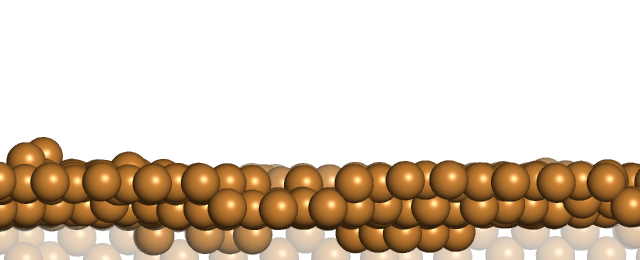
\includegraphics[width=\textwidth]{Cu_crater_01_crop}
    \subcaption{$t=59$}
  \end{subfigure}
  \hfill
  \begin{subfigure}[t]{\subfigwidth}
    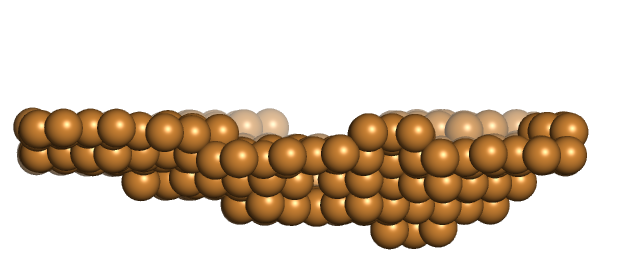
\includegraphics[width=\textwidth]{Cu_crater_07_crop}
    \subcaption{$t=65$}
  \end{subfigure}
  \hfill
  \begin{subfigure}[t]{\subfigwidth}
    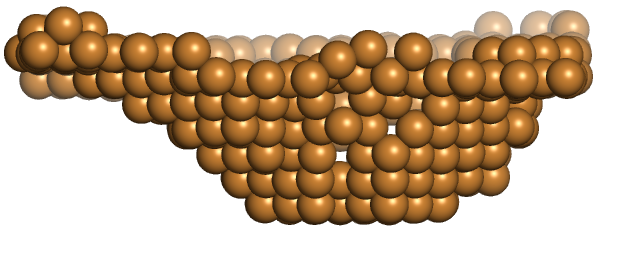
\includegraphics[width=\textwidth]{Cu_crater_17_crop}
    \subcaption{$t=75$}
  \end{subfigure}

  \begin{subfigure}[t]{\subfigwidth}
    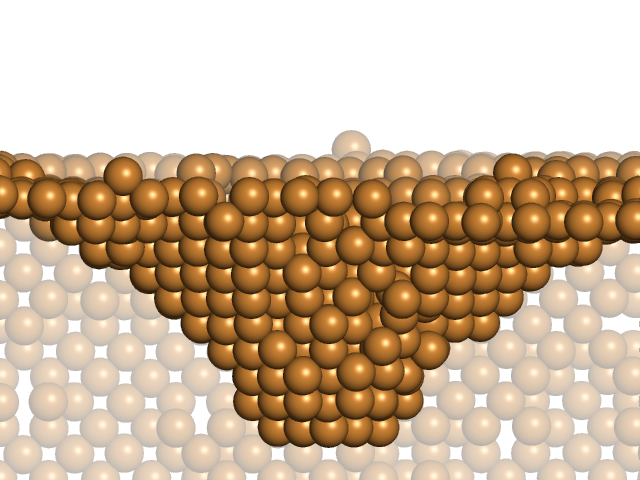
\includegraphics[width=\textwidth]{Cu_crater_27}
    \subcaption{$t=85$}
  \end{subfigure}
  \hfill
  \begin{subfigure}[t]{\subfigwidth}
    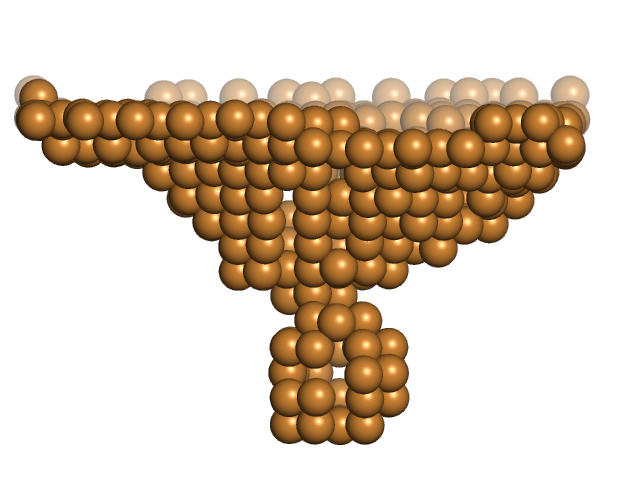
\includegraphics[width=\textwidth]{Cu_crater_37}
    \subcaption{$t=95$}
  \end{subfigure}
  \hfill
  \begin{subfigure}[t]{\subfigwidth}
    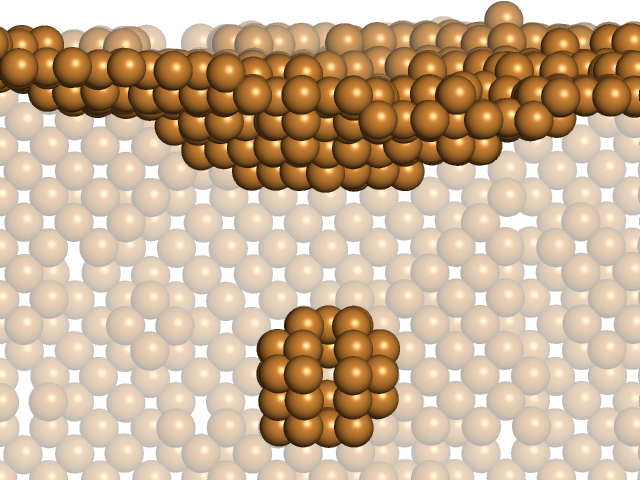
\includegraphics[width=\textwidth]{Cu_crater_42}
    \subcaption{$t=100$}
  \end{subfigure}

  \caption[Bildung und Abschluss eines Kupfer-Kraters]{
    Bildung und Abschluss eines Kupfer-Kraters mit \pot{u3}.\\
    Seitenansicht der extrahierten Oberflächenatome
  }
  \label{fig:coppercrater}
\end{figure}

\subsection{Untersuchung der maximalen Workerdichte}

Ergänzend ist in Abbildung~\ref{fig:copperworkerdensity-b} ein Histogramm der Zahl paralleler Ereignisse dargestellt, aus der auf die Workerdichte geschlossen werden kann\todo{hier findet keine Limitierung durch die Zahl der verfügbaren Kerne statt?}.
Die Verteilung hat ihren Mittelwert bei $p = \num{6.3}$ mit dem Maximum von aktiven Prozessen bei $p_\text{peak} = \num{13}$, wobei der Hauptprozess bereits zu $p$ gezählt wurde.
Dem steht eine analytisch ermittelte maximale Zahl von Prozessen mit $p_\text{max} = \num{30}$ gegenüber, die allerdings eine dichte Packung von MD-Boxen auf der Oberfläche voraus setzt.
Durch die zufällige Auswahl der Ereignisorte und der Bewahrung der Reihenfolge der Ereignisse ergeben sich in Parsivald-Simulationen vergleichsweise effiziente Workerdichten von $\rho_\text{worker} = \SI{18.5}{\percent}$.

\begin{figure}

  \captionsetup[subfigure]{justification=centering,singlelinecheck=false}
  \def\subfigwidth{7cm}

  \begin{subfigure}[t]{\subfigwidth}
    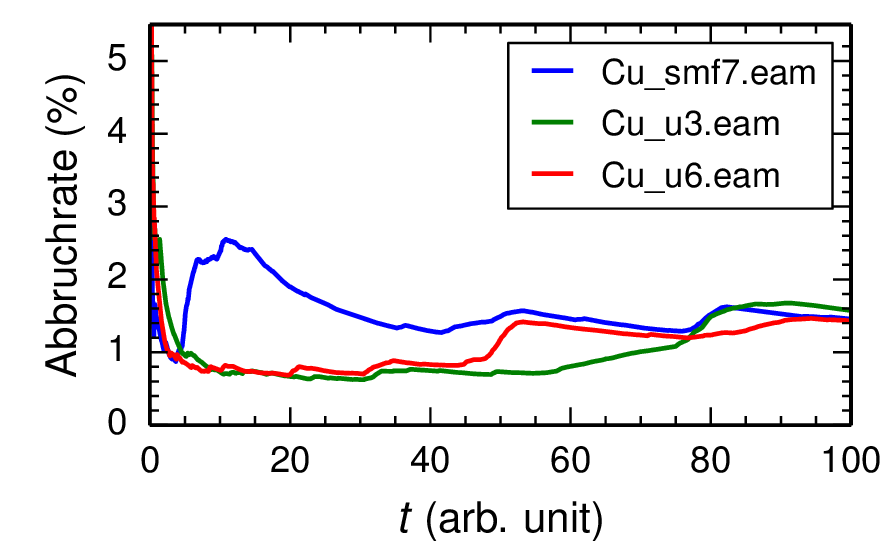
\includegraphics[width=\textwidth]{Cu_abortstatplot}
    \subcaption{Abbruchraten von Kupfer-Simulationen}
    \label{fig:copperworkerdensity-a}
  \end{subfigure}
  \hfill
  \begin{subfigure}[t]{\subfigwidth}
    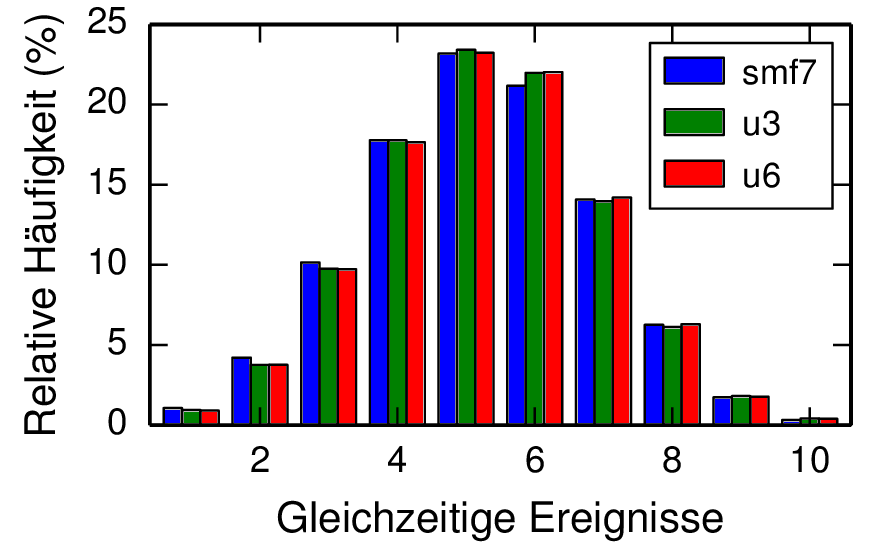
\includegraphics[width=\textwidth]{Cu_eventhistogram}
    \subcaption{Histogramm gleichzeitiger Ereignisse}
    \label{fig:copperworkerdensity-b}
  \end{subfigure}
  \caption{Simulationen von Kupfer-PVD auf \SI{200x200x24}{\angstrom} großen Substraten}
  \label{fig:copperworkerdensity}
\end{figure}
